\mychapter{ئالدىن بىلىملەر}
\par\bigskip
\begin{tcolorbox}
بۇ باپتا ئالىي ماتېماتىكا ئۆگىنىشتىن ئاۋال ھازىرلاشقا تىگىشلىك ئالدىن بىلىملەر خاتېرلەندى. بۇ بىلىملەر ئوتتۇرا مەكتەپ ماتىماتىكا بىلىملىرىدىن ئالىي ماتېماتىكا بىلىملىرىگە بولغان ئۆتكۈنچى نۇقتىلار ھېساپلىنىدۇ.
\end{tcolorbox}

\section{فۇنكىسىيە}
فۇنكسىيەنىڭ ئېنىقلىمىسى ئادەتتە ئەنئەنىۋى ئېنىقلىما ۋە زامانىۋى ئېنىقلىما دەپ ئىككىگە بۆلىنىدۇ. باياننىڭ ئۇقۇمىنىڭ باشلىنىش نۇقتىسى باشقىچە بولغاندىن باشقا ، فۇنكىسىيەنىڭ ئىككى ئېنىقلىمىسى ئاساسەن ئوخشاش. ئەنئەنىۋى ئېنىقلىما ھەرىكەت ئۆزگىرىشى نۇقتىسىدىن باشلىنىدۇ. ، زامانىۋى ئېنىقلىما بولسا توپلام ۋە ئەكىس ئېتىش نۇقتىسىدىن باشلىنىدۇ.

\subsection{ئاساسىي ئېلېمېنتار فۇنكسىيە }
ئاساسىي ئېلېمېنتار فۇنكسىيە تۇراقلىق سان فۇنكسىيەسى، دەرىجە فۇنكسىيەسى، كۆرسەتكۈچلۈك فۇنكسىيە، لوگارىفمىلىق فۇنكسىيە، ترىگونومېتىرىيەلىك فۇنكسىيە، تەتۈر ترىگونومېتىرىيەلىك فۇنكسىيەنى ئۆز ئىچىگە ئالىدۇ. تەپسىلاتى تۆۋەندىكىچە:

تۇراقلىق سان فۇنكسىيەسى
بىرىنچى دەرىجىلىك فۇنكسىيە
ئىككىنچى دەرىجىلىك فۇنكسىيە
تەتۈر تاناسىپلىق فۇنكىسىيە
دەرىجىلىك فۇنكسىيە
كۆرسەتكۈچلۈك فۇنكسىيە
لوگارىفمىلىق فۇنكسىيە
ترىگونومېتىرىيەلىك فۇنكسىيە
تەتۈر ترىگونومېتىرىيەلىك فۇنكسىيە

\subsubsection{تۇراقلىق سان فۇنكسىيەسى}\par\bigskip
%\begin{minipage}{0.35\linewidth}
$y=f(x)=C$ بۇنىڭدا $C$ تۇراقلىق سان. 
%\end{minipage}

\subsubsection{بىرىنچى دەرىجىلىك فۇنكسىيە}
$y=f(x)=ax+b$,$a,b$ خالىغان سان، ھەم
$a \neq 0$

\subsubsection{ئىككىنچى دەرىجىلىك فۇنكسىيە}
$y=f(x)=ax^2+bx+c$,$a,b,c$ خالىغان سان، ھەم
$a \neq 0$

\subsubsection{تەتۈر تاناسىپلىق فۇنكىسىيە}
$y=f(x)=\frac{a}{x}$,$a$ خالىغان سان.

\subsubsection{دەرىجىلىك فۇنكسىيە}\par\bigskip
$y=x^{\mu}$، $\mu$ خالىغان سان\\
$x>0$، $y=x^{\mu}$ رەسىمدىكىدەك بولىدۇ.
\begin{center}
\begin{tikzpicture}[scale=0.9]
        \draw[-latex](-2,0) -- (2,0) node[below]{$x$};
        \draw[-latex](0,-2) -- (0,4) node[above]{$y$};
        \draw[black, thick, smooth, domain=0.3:2] plot (\x,1/\x) node[right]{$\mu =-1$};
        \draw[black, thick, smooth, domain=-2:-0.5] plot (\x,1/\x) node[right]{$\mu =-1$};
        \draw[black, thick, smooth, domain=0.01:2] plot (\x, {sqrt(\x)});
        \filldraw[black] (2.75,1.25) node {$\mu =\dfrac{1}{2}$};
        \draw[black, thick, smooth, domain=-2:2] plot (\x,\x) node[right]{$\mu =1$};
        \draw[black, thick, smooth, domain=-2:2] plot (\x, {\x*\x}) node[right]{$\mu =2$};
        \filldraw[black] (0,0) node[below]{$O$};
        \filldraw[black] (1,1) circle (2pt) node at(1.25,0.5){$(1,1)$};
    \end{tikzpicture}
\end{center}

\subsubsection{كۆرسەتكۈچلۈك فۇنكسىيە}\par\bigskip%
$y=a^x(a>0,a\neq 1)$
\begin{center}
    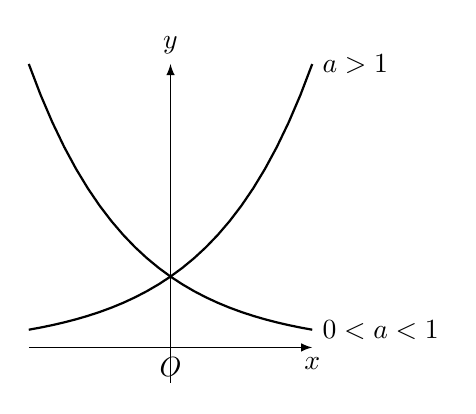
\begin{tikzpicture}[scale=0.9]
        \draw[-latex](-2,0) -- (2,0) node[below]{$x$};
        \draw[-latex](0,-0.5) -- (0,4) node[above]{$y$};
        \draw[black, thick, domain=-2:2] plot (\x,{pow(1/2,\x)}) node[right]{$0<a<1$};
        \draw[black, thick, domain=-2:2] plot (\x,{pow(2,\x)}) node[right]{$a>1$};
        \filldraw[black] (0,0) node[below]{$O$};
    \end{tikzpicture}
\end{center}

\subsubsection{لوگارىفمىلىق فۇنكسىيە}\par\bigskip
$y=log_ax(a>0,a\neq 1)$
\begin{center}
    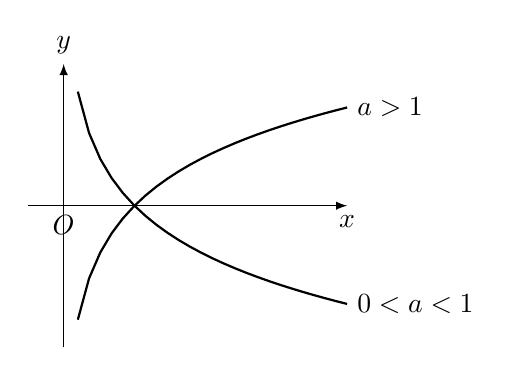
\begin{tikzpicture}[scale=0.9]
        \draw[-latex](-0.5,0) -- (4,0) node[below]{$x$};
        \draw[-latex](0,-2) -- (0,2) node[above]{$y$};
        \draw[black, thick, domain=0.2:4] plot (\x,{ln(1/\x)}) node[right]{$0<a<1$};
        \draw[black, thick, domain=0.2:4] plot (\x,{ln(\x)}) node[right]{$a>1$};
        \filldraw[black] (0,0) node[below]{$O$};
    \end{tikzpicture}
\end{center}

\subsubsection{ترىگونومېتىرىيەلىك فۇنكسىيە}\par\bigskip
سىنوس فۇنكىسىيەسى:
\begin{center}
\begin{tikzpicture}[scale=0.9]
    \draw[-latex](-5,0) -- (5,0) node[below]{$x$};
    \draw[-latex](0,-1.5) -- (0,2) node[above]{$y$};
    \draw[black, thick, smooth, domain=-5:5] plot (\x,{sin(\x r)}) node at (0,1.5){$\sin(x)$};
    \draw[black, densely dashed](-5,1) -- (5,1) node[right]{$x=1$};
    \draw[black, densely dashed](-5,-1) -- (5,-1) node[right]{$x=-1$};
    \draw[black, densely dashed](-pi/2*3,1) -- (-pi/2*3,0) node[below]{$-\dfrac{3\pi}{2}$};
    \draw[black, densely dashed](-pi/2,-1) -- (-pi/2,0) node[above]{$-\dfrac{\pi}{2}$};
    \draw[black, densely dashed](pi/2,1) -- (pi/2,0) node[below]{$\dfrac{\pi}{2}$};
    \draw[black](0,0) -- (0,0) node[above]{$O$};
    \filldraw[black] (-pi-0.1,0) node[below]{$-\pi$};
    \filldraw[black] (pi,0) node[below]{$\pi$};
\end{tikzpicture}
\end{center}
كوسىنۇس فۇنكسىيەسى:
\begin{center}
\begin{tikzpicture}[scale=0.9]
    \draw[-latex](-5,0) -- (5,0) node[below]{$x$};
    \draw[-latex](0,-1.5) -- (0,2) node[above]{$y$};
    \draw[black, thick, smooth, domain=-5:5] plot (\x,{cos(\x r)}) node at (0,1.5){$\cos(x)$};
    \draw[black, densely dashed](-5,1) -- (5,1) node[right]{$x=1$};
    \draw[black, densely dashed](-5,-1) -- (5,-1) node[right]{$x=-1$};
    \draw[black, densely dashed](-pi,-1) -- (-pi,0) node[above]{$-\pi$};
    \draw[black, densely dashed](pi,-1) -- (pi,0) node[above]{$\pi$};
    \filldraw[black] (0,0) node[below]{$O$};
    \filldraw[black] (-pi/2*3-0.25,0) node[below]{$-\dfrac{3\pi}{2}$};
    \filldraw[black] (-pi/2,0) node[below]{$-\dfrac{\pi}{2}$};
    \filldraw[black] (pi/2,0) node[below]{$\dfrac{\pi}{2}$};
\end{tikzpicture}
\end{center}
تانگېنىس فۇنكىسيەسى:
\begin{center}
\begin{tikzpicture}[scale=0.55]
        \draw[-latex](-6,0) -- (6,0) node[below]{$x$};
        \draw[-latex](0,-2) -- (0,2) node[above]{$y$};
        \draw[black, thick, domain=-pi/2+0.5:pi/2-0.5] plot (\x,{tan(\x r)}) node[above]{$\tan(x)$};
        \draw[black, densely dashed](pi/2,2) -- (pi/2,-2);
        \draw[black, densely dashed](-pi/2,2) -- (-pi/2,-2);
        \draw[black, thick, domain=-pi/2*3+0.5:-pi/2-0.5] plot (\x,{tan(\x r)}) node[above]{$\tan(x)$};
        \draw[black, densely dashed](pi/2*3,2) -- (pi/2*3,-2);
        \draw[black, thick, domain=pi/2+0.5:pi/2*3-0.5] plot (\x,{tan(\x r)}) node[above]{$\tan(x)$};
        \draw[black, densely dashed](-pi/2*3,2) -- (-pi/2*3,-2);
        \filldraw[black] (0,0) node[below]{$O$};
        \filldraw[black] (pi/2+0.5,-0.75) node{$\dfrac{\pi}{2}$};
        \filldraw[black] (-pi/2-0.75,-0.75) node{$-\dfrac{\pi}{2}$};
        \filldraw[black] (pi/2*3+0.5,-0.75) node{$\dfrac{3\pi}{2}$};
        \filldraw[black] (-pi/2*3-0.75,-0.75) node{$-\dfrac{3\pi}{2}$};
    \end{tikzpicture}
\end{center}
كوتانگېنىس فۇنكسيەسى:
\begin{center}
\begin{tikzpicture}[scale=0.65]
        \draw[-latex](-4,0) -- (4,0) node[below]{$x$};
        \draw[-latex](0,-2) -- (0,2) node[above]{$y$};
        \draw[black, thick, domain=0.5:pi-0.5] plot (\x,{cot(\x r)}) node at(pi-1,2){$\cot(x)$};
        \draw[black, densely dashed](pi,2) -- (pi,-2);
        \draw[black, thick, domain=-0.5:-pi+0.5] plot (\x,{cot(\x r)}) node at(-1,2){$\cot(x)$};
        \draw[black, densely dashed](-pi,2) -- (-pi,-2);
        \filldraw[black] (0,0) node[below]{$O$};
        \filldraw[black] (pi/2,0) node[below]{$\dfrac{\pi}{2}$};
        \filldraw[black] (pi+0.5,-0.5) node{$\pi$};
        \filldraw[black] (-pi/2-0.25,0) node[below]{$-\dfrac{\pi}{2}$};
        \filldraw[black] (-pi-0.5,-0.5) node{$-\pi$};
    \end{tikzpicture}
\end{center}

\subsubsection{تەتۈر ترىگونومېتىرىيەلىك فۇنكسىيە}\par\bigskip

دددددد

\subsection{ترىگونومېتىرىيەلىك فۇنكسىيەلەر فورمۇلاسى}
يىغىندى:\\
\begin{align*}
    \sin \alpha \cos \beta & =\frac{1}{2}[\sin (\alpha+\beta)+\sin(\alpha-\beta)]  \\[7pt]
    \cos \alpha \sin \beta & =\frac{1}{2}[\sin (\alpha+\beta)-\sin(\alpha-\beta)]  \\[7pt]
    \cos \alpha \cos \beta & =\frac{1}{2}[\cos (\alpha+\beta)+\cos(\alpha-\beta)]  \\[7pt]
    \sin \alpha \sin \beta & =-\frac{1}{2}[\cos (\alpha+\beta)-\cos(\alpha-\beta)]
\end{align*}
كۆپەيمە:
\begin{align*}
    \sin\alpha+\sin\beta & =2\sin\frac{\alpha+\beta}{2}\cos\frac{\alpha-\beta}{2}  \\[7pt]
    \sin\alpha-\sin\beta & =2\cos\frac{\alpha+\beta}{2}\sin\frac{\alpha-\beta}{2}  \\[7pt]
    \cos\alpha+\cos\beta & =2\cos\frac{\alpha+\beta}{2}\cos\frac{\alpha-\beta}{2}  \\[7pt]
    \cos\alpha-\cos\beta & =-2\sin\frac{\alpha+\beta}{2}\sin\frac{\alpha-\beta}{2} \\[7pt]
    \tan\alpha+\tan\beta & =\frac{\sin (\alpha+\beta)}{\cos\alpha\cdot\cos \beta}
\end{align*}

بىرلىك:\\
\begin{align*}\label{gyhgs}
    \sin^2 x+\cos^2x  & =1 \\[7pt]
    \sec^2 x-\tan^2x  & =1 \\[7pt]
    \cosh^2x-\sinh^2x & =1
\end{align*}
يېرىم بۇلۇڭ:\\
\begin{align*}
    \sin^2x & =\frac{1}{2}(1-\cos 2x)                                                        \\[7pt]
    \cos^2x & =\frac{1}{2}(1+\cos 2x)                                                        \\[7pt]
    \tan^2x & =\frac{1-\cos 2x}{1+\cos 2x}                                                   \\[7pt]
    \sin x  & =2\sin\frac{x}{2}\cos\frac{x}{2}                                               \\[7pt]
    \cos x  & =2\cos^2\frac{x}{2}-1=1-2\sin^2\frac{x}{2}=\cos^2\frac{x}{2}-\sin^2\frac{x}{2} \\[7pt]
    \tan x  & =\frac{2\tan(x/2)}{1-\tan^2(x/2)}
\end{align*}

\subsection{ھاسىلە فورمۇلاسى}
\begin{multicols}{3}
    \begin{equation*}
        \left( C\right)'=0
    \end{equation*}
    \begin{equation*}
        \left( x^{\mu}\right)'=\mu x^{\mu-1}
    \end{equation*}
    \begin{equation*}
        \left( \sin x\right)'=\cos x
    \end{equation*}
    \begin{equation*}
        \left( \cos x\right)'=-\sin x
    \end{equation*}
    \begin{equation*}
        \left( \tan x\right)'=\sec^2 x
    \end{equation*}
    \begin{equation*}
        \left( \cot x\right)'=-\csc^2 x
    \end{equation*}
    \begin{equation*}
        \left( \sec x\right)'=\sec x\cdot\tan x
    \end{equation*}
    \begin{equation*}
        \left( \csc x\right)'=-\csc x\cdot\tan x
    \end{equation*}
    \begin{equation*}
        \left( a^x\right)'=a^x\ln a\ (a>0,a\neq1)
    \end{equation*}
    \begin{equation*}
        \left( \log_{a}x\right)'=\frac{1}{x\cdot\ln a}\ (a>0,a\neq1)
    \end{equation*}
    \begin{equation*}
        \left( \arcsin x\right)'=\frac{1}{\sqrt{1-x^2}}
    \end{equation*}
    \begin{equation*}
        \left( \arccos x\right)'=-\frac{1}{\sqrt{1-x^2}}
    \end{equation*}
    \begin{equation*}
        \left( \arctan x\right)'=\frac{1}{1+x^2}
    \end{equation*}
    \begin{equation*}
        \left( \mathrm{arccot}\, x\right)'=-\frac{1}{1+x^2}
    \end{equation*}
\end{multicols}

\subsection{ئىنتېگىرال فورمۇلاسى}
\begin{align*}
     & \int x^\mu\,\mathrm{d}x=\frac{x^{\mu+1}}{\mu+1}+C\ (\mu\neq-1)                                                         \\[7pt]
     & \int \frac{1}{x}\,\mathrm{d}x=\ln|x|+C                                                                                 \\[7pt]
     & \int\frac{\mathrm{d}x}{1+x^2}=\arctan x+C                                                                              \\[7pt]
     & \int\frac{\mathrm{d}x}{\sqrt{1-x^2}}=\arcsin x+C_1=-\arccos x+C_2                                                      \\[7pt]
     & \int \sin x\,\mathrm{d}x=-\cos x+C                                                                                     \\[7pt]
     & \int\cos x \,\mathrm{d}x=\sin x +C                                                                                     \\[7pt]
     & \int\tan x\,\mathrm{d}x=-\ln |\cos x|+C                                                                                \\[7pt]
     & \int\cot x\,\mathrm{d}x=\ln |\sin x|+C                                                                                 \\[7pt]
     & \int\csc x\,\mathrm{d}x=\int\frac{1}{\sin{x}}\,\mathrm{d}x=\frac{1}{2}
    \ln{\left|\frac{1-\cos{x}}{1+\cos{x}}\right|}+C=\ln{\left|\tan{\frac{x}{2}}\right|}+C=\ln{\left|\csc{x}-\cot{x}\right|}+C \\[7pt]
     & \int\sec x\,\mathrm{d}x=\int\frac{1}{\cos{x}}\,\mathrm{d}x=\frac{1}{2}
    \ln{\left|\frac{1+\sin{x}}{1-\sin{x}}\right|}+C=\ln{\left|\sec{x}+\tan{x}\right|}+C                                       \\[7pt]
     & \int\sec^2 x\,\mathrm{d}x=\tan x +C                                                                                    \\[7pt]
     & \int \csc^2 x\,\mathrm{d}x=-\cot x +C                                                                                  \\[7pt]
     & \int \sec x\cdot\tan x \,\mathrm{d}x=\sec x+C                                                                          \\[7pt]
     & \int\csc x \cdot\cot x \,\mathrm{d}x=-\csc x+C                                                                         \\[7pt]
     & \int \mathrm{e}^x \,\mathrm{d}x=\mathrm{e}^x+C                                                                         \\[7pt]
     & \int a^x\,\mathrm{d}x=\frac{a^x}{\ln a}+C                                                                              \\[7pt]
     & \int \sinh x\,\mathrm{d}x=\cosh x+C                                                                                    \\[7pt]
     & \int \cosh x\,\mathrm{d}x=\sinh x+C                                                                                    \\[7pt]
     & \int \frac{1}{a^2+x^2}\,\mathrm{d}x=\frac{1}{a}\arctan\frac{x}{a}+C                                                    \\[7pt]
     & \int \frac{1}{a^2-x^2}\,\mathrm{d}x=\frac{1}{2a}\ln \left|\frac{a+x}{a-x}\right|+C                                     \\[7pt]
     & \int \frac{1}{\sqrt{a^2-x^2}}\,\mathrm{d}x=\arcsin\frac{x}{a}+C                                                        \\[7pt]
     & \int \frac{1}{\sqrt{x^2\pm a^2}}\,\mathrm{d}x=\ln \left|x+\sqrt{x^2\pm a^2}\right|+C
\end{align*}

\section{سانلار ئارقىمۇ ئارقىلىقى}
\subsection{تەڭ ئايرىمىلىق سانلار ئارقىمۇ ئارقىلىقى}

\subsection{تەڭ نىسبەتلىك سانلار ئارقىمۇ ئارقىلىقى}

\subsection{سانلار قاتارى}

\subsection{سانلار قاتارى يىغىندىسى}
\begin{english}
\begin{enumerate}
    \item $\sum_{k=1}^nk=1+2+\cdots+n=\dfrac{n(n+1)}{2}$
    \item $\sum_{k=1}^nk^2=1^2+2^2+\cdots+n^2=\dfrac{n(n+1)(2n+1)}{6}$
    \item $\sum_{k=1}^n\dfrac{1}{k(k+1)}=\dfrac{1}{1\times 2}+\dfrac{1}{2\times 3}+\cdots+\dfrac{1}{n(n+1)}=\dfrac{n}{n+1}$
\end{enumerate}
\end{english}

دەرىجە فۇنكسىيەسىگە نىسبەتەن ئوخشاش بولمىغان دەرىجە ئاستىدىكى ئوخشاش مونوتونلۇققا ئاساسەن ئەڭ قىممەتنى تەتقىق قىلىشقا بولىدۇ





